\documentclass[../../main.tex]{subfiles}
\begin{document}

{\bf [解]}

(1)
準線のうち $x > 0$ のものを $l$ とする. 焦点の座標が $F(ae, 0)$ だから，この楕円の離心率は $e$ である．
下図のように楕円上の点 $P$，および$P$ から$l$におろした垂線の足を $H$ を定める．
また$l$と$x$軸の交点を$I$とする．

\begin{figure}[htb]
 \begin{center}
 \begin{tikzpicture}[scale=2, >=stealth]
  % 1. 各パラメータの決定 (a=1.5, b=1.0)
  % e = sqrt(1 - b^2/a^2) = sqrt(1 - 1/2.25) = sqrt(5)/3 ≈ 0.745356
  % c = ae = sqrt(a^2 - b^2) = sqrt(1.25) ≈ 1.11803
  % a/e ≈ 2.01246
  
  \coordinate (O) at (0,0);
  \coordinate (F) at (1.11803, 0); % 焦点 (ae, 0)

  % θ = 50度における焦点からの距離 r = l / (1 + e*cos θ)
  % ここで 半半弦 l_param = b^2 / a = 1.0 / 1.5 = 2/3 ≈ 0.66667
  % r = (2/3) / (1 + 0.745356 * cos(50°)) ≈ 0.45075
  % したがって P の座標は (ae + r*cos 50°, r*sin 50°)
  \coordinate (P) at ({1.11803 + 0.45075*cos(50)}, {0.45075*sin(50)});
  \coordinate (H) at (2.01246, {0.45075*sin(50)});
  \coordinate (I) at (2.01246, 0);

  % Axes
  \draw[->] (-1.8,0) -- (2.5,0) node[below] {$x$};
  \draw[->] (0,-1.4) -- (0,1.4) node[left] {$y$};
  \node[below left] at (O) {$O$};

  % Ellipse (a=1.5cm, b=1.0cm)
  \draw[thick] (0,0) ellipse (1.5cm and 1.0cm);

  % Points and ticks
  \fill (F) circle (1pt) node[above left] {$F$};
  \node[below, yshift=-2pt] at (1.11803,0) {\small $ae$};
  \node[below left] at (1.5,0) {$a$};
  \node[above left] at (0,1.0) {$b$};

  % Directrix l (x = a/e)
  \draw[dashed, thick] (2.01246,-1.3) -- (2.01246,1.3) node[above] {$l$};
  \node[below right] at (2.01246,0) {$\dfrac{a}{e}$};

  % Segments and Points (P, H)
  \draw[thick] (F) -- (P) node[midway, left] {$r$};
  \draw[thick] (P) -- (H);
  \draw[dotted] (P) -- ({1.11803 + 0.45075*cos(50)}, 0); % Pからの垂線

  \fill (P) circle (1pt) node[above right] {$P$};
  \fill (H) circle (1pt) node[above right] {$H$};
  \fill (I) circle (1pt) node[above right] {$I$};


  % Angle theta arc
  \draw (1.11803+0.2,0) arc (0:50:0.2);
  \node at (1.11803+0.3, 0.1) {\small $\theta$};

  % 垂直記号 (H)
  \draw (1.91246, {0.45075*sin(50)}) -- (1.91246, {0.45075*sin(50)-0.1}) -- (2.01246, {0.45075*sin(50)-0.1});
 \end{tikzpicture}
 \caption{楕円と焦点 $F$，準線 $l$ の関係}
 \end{center}
\end{figure}


焦点と準線の性質から
\begin{align}
    |PF| = e |PH| \label{eq:1}
\end{align}
である．$|FI|$を二通りの長さで表すと
\begin{align}
 |FP|\cos\theta + |PH| = |FI| \label{eq:2}
\end{align}
である．極座標を$P(r,\theta)$とすると各長さは\cref{eq:1}にも注意して
\begin{align}
 |PF| &= r \\
 |PH| &= \dfrac{r}{e} \\
 |FI| &= \dfrac{a}{e} - ae 
\end{align}
と書けるから\cref{eq:2}に代入して
\begin{align}
 \dfrac{a}{e} - ae = r \cos \theta + \dfrac{r}{e} \\
 \therefore   
r = \dfrac{a(1-e^2)}{1+e\cos\theta}
\end{align}
が求める方程式である．


(2)
線分$PQ$，$RS$が点$F$を通ってかつこれら二つが直交するので，$P, Q$ に対応する $\theta$ を $\alpha, \alpha+\pi \, (0 \leqq \alpha \leqq \pi)$, $R, S$ に対応する $\theta$ を $\alpha-\dfrac{\pi}{2}, \alpha+\dfrac{\pi}{2}$ とおける．
簡単のため$A = a(1-e^2)$ とすると各線分の長さは
\begin{align}
 |PF| \cdot |QF| &= r(\alpha) \cdot r(\alpha+\pi) \\
  &= \dfrac{A}{1+e\cos\alpha} \cdot \dfrac{A}{1-e\cos\alpha} = \dfrac{A^2}{1-e^2\cos^2\alpha} \\
 |FR| \cdot |FS| &= r\left(\alpha+\dfrac{\pi}{2}\right) r\left(\alpha-\dfrac{\pi}{2}\right) = \dfrac{A^2}{1-e^2\sin^2\alpha}
\end{align}
だから求める値は
\begin{align}
 \dfrac{1}{|PF|\cdot|QF|} + \dfrac{1}{|FR|\cdot|FS|} = \dfrac{2-e^2}{A^2} = \dfrac{2-e^2}{a^2(1-e^2)^2}.
\end{align}
である．

\begin{figure}[htb]
\begin{center}
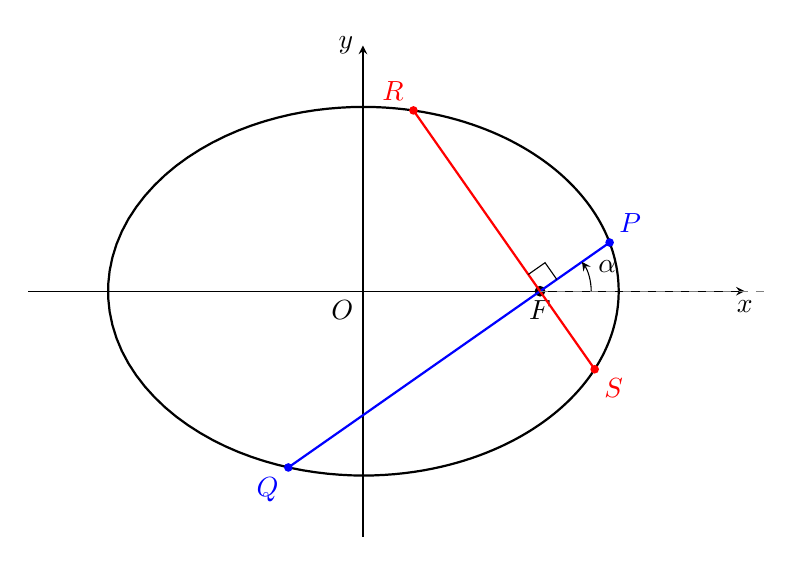
\begin{tikzpicture}[scale=1.3, >=stealth]
  % 媒介変数表示による楕円の描画 (中心 (c,0), 長半径 a=2.5, 短半径 b=1.8, 焦点 c=sqrt(a^2-b^2)≒1.73)
  % ここでは焦点 F を原点 (0,0) とした極座標形式で描画
  % e = 0.692, A = a(1-e^2) ≒ 1.3
  \draw[thick, domain=0:360, samples=200] 
    plot ({1.3/(1 + 0.692*cos(\x))*cos(\x)}, {1.3/(1 + 0.692*cos(\x))*sin(\x)});

  % 焦点 F（原点）
  \coordinate (F) at (0,0);
  \fill (F) circle (1.5pt) node[below] {$F$};

  % 角度 alpha の設定 (例: 35度)
  \def\alphaVal{35}

  % 焦点 F から各点 P, Q, R, S への極座標計算
  % P: theta = alpha
  % Q: theta = alpha + 180
  % R: theta = alpha + 90
  % S: theta = alpha - 90
  \coordinate (P) at ({\alphaVal}:{1.3/(1 + 0.692*cos(\alphaVal))});
  \coordinate (Q) at ({\alphaVal+180}:{1.3/(1 - 0.692*cos(\alphaVal))});
  \coordinate (R) at ({\alphaVal+90}:{1.3/(1 - 0.692*sin(\alphaVal))});
  \coordinate (S) at ({\alphaVal-90}:{1.3/(1 + 0.692*sin(\alphaVal))});

  % Axes
  \draw[->] (-5,0) -- (2,0) node[below] {$x$};
  \draw[->] (-1.73,-2.4) -- (-1.73,2.4) node[left] {$y$};
  \node[below left] at (-1.73,0) {$O$};

  % 弦 PQ と 弦 RS の描画
  \draw[thick, blue] (P) -- (Q);
  \draw[thick, red] (R) -- (S);

  % 各点の頂点ラベル
  \fill[blue] (P) circle (1.2pt) node[above right] {$P$};
  \fill[blue] (Q) circle (1.2pt) node[below left] {$Q$};
  \fill[red] (R) circle (1.2pt) node[above left] {$R$};
  \fill[red] (S) circle (1.2pt) node[below right] {$S$};

  % 始線 (x軸方向) の参考破線
  \draw[dashed, gray] (F) -- (2.2, 0);

  % 角度 alpha の表示
  \draw[->] (0.5,0) arc (0:\alphaVal:0.5);
  \node at (20:0.7) {$\alpha$};

  % 直角マーク (F における PQ と RS の直交)
  \begin{scope}[rotate=\alphaVal]
    \draw (0.2,0) -- (0.2,0.2) -- (0,0.2);
  \end{scope}

\end{tikzpicture}
\end{center}
\caption{焦点 $F$ を通り直交する2つの弦 $PQ$ と $RS$}
\end{figure}


\end{document}
